\input{chapter-header.tex}
% ===========================================================================
\part{Tailoring: Automatic Extraction of Application Runtimes}
% ===========================================================================
\chapter{Run-Fail-Grow: a Dynamic Approach}
\chaplabel{chap:rfg}
\minitoc
% ===========================================================================
\introduction
% ===========================================================================



This chapter describes the \emph{run-fail-grow} (RFG) technique: an alternative solution to dead code elimination that identifies the code units that are actually used in an application during runtime~(Section~\ref{sec:rfg_model}).
Using RFG, we launch a \emph{reference} application containing all code units~(base libraries, third party libraries and application code) and a \emph{nurtured} application runtime containing a \emph{seed} \ie a minimal set of code units we want to ensure in our application.
RFG generates an application runtime by ``growing'' the nurtured application into a deployable specialized version of the reference application. 
RFG runs the nurtured version of the application and feeds it with the code units that were detected as missing with a failure~(Section \ref{sec:rfg_example}).

The resulting deployable application only embeds the seed and used code.
By carefully choosing the seed, the user configures the scope of the tailoring process making possible different levels of tailoring.
For example, a seed that includes all base libraries makes the tailoring process to only select used code in the application-specific part; whereas an empty seed makes the tailoring process to select used code in all parts: base libraries, application libraries and application-specific part~(Section \ref{sec:seeds}).
% For example, if the seed includes the language base libraries, it ensures that the deployed application will have it all whereas an empty seed will result that only part of the base libs 
% Afterwards, deployment units are created from this shrank application to only contain the used code units.
% Using these compacted deployment units leverages the targeted device limitations. 

The dynamic nature of our solution allows its usage in dynamically-typed languages, and applications using reflection. Our solution does not need to modify the original application thanks to its run-fail-grow approach.
It also successfully deals with applications that make use of programming language features such as reflection or open classes.

We developed Tornado, an RFG implementation using \Vtt~(Section~\ref{sec:rfg_implementation}). In Tornado, the nurtured application resides inside a virtualized runtime. With \Vtt, we can monitor the execution of the nurtured application to detect whether a code unit is missing or not. Using \Vtt's mirrors we can also install the required code units.

\section{Run Fail Grow: Dynamic dead code elimination}\label{sec:rfg_model}

We propose a tailoring technique we named run-fail-grow~(RFG). Briefly, RFG works by launching a \emph{reference} application encompassing the full application with all its code units~(base libraries, third party libraries and application code) and a \emph{nurtured} application that has only part of its required code units installed. The nurtured application is run, and when a failure is detected because it misses a code unit, we install into it the corresponding code unit from the reference application. Thus, the nurtured application grows progressively as missing code units are found and solved.
Once finished, the nurtured application is ready to be deployed on target devices. Figure~\ref{fig:runfail} depicts the basics of our run-fail-grow approach.

\begin{figure}[ht]
\begin{center}
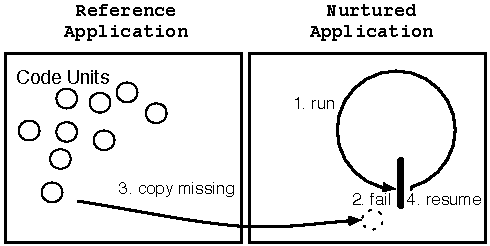
\includegraphics[width=.7\linewidth]{runfail}
\caption{\small \textbf{Application tailoring with a run-fail-grow approach.} We~(1) run the nurtured application and~(2) detect the missing units on failure. For each failure,~(3) we copy missing code units from the reference application and then~(4) the execution is resumed (just before the failure point) until the process finishes. \label{fig:runfail}}
\end{center}
\end{figure}

On one side, we start the reference application and pause it at the point where either it contains all its collection of code units, either we can load them dynamically~(under a lazy loading strategy). The reference application remains paused to avoid to mutate its state during the tailoring process. Pausing consists in suspending all processes and threads from the application.

On the other side, we fill initially the nurtured application with the \emph{seed} \ie the set of code units that we want to ensure in the final application. This seed allows us to specify the level of specialization of our deployable application.
By using a seed that contains all base libraries, RFG will only affect the application specific code units and third-party libraries.
However, by using an empty seed, it will also tailor base libraries~(cf. Section \ref{sec:seeds}).

Running the nurtured application consists in two main steps. We first install in the nurtured application one or more \emph{application's entry points} in the form of threads, and then we start to run it.
The execution of these entry points results into sending messages to those objects that start the application. These messages will produce \emph{missing code failures} when the respective classes and methods to resolve the message are not available.
We detect the missing code failures and solve them by fetching the needed code units from the reference application and install them into the nurtured application. RFG installs only code units on demand \ie the content of installed classes and objects is not installed with them but deferred until it is actually needed; methods are not installed until they are invoked.
The process repeats until we end it explicitly, so we can interact with the application as part of the process. Ideally, the nurtured application reaches a stable point where it needs no more code units.
The nurtured application is then ready for deployment.

The dynamic nature of RFG tackles all our challenges. Missing code units are detected and resolved at runtime, where two main elements are available: the exact messages that are sent with their corresponding receiver and arguments, and their concrete types\footnote{We consider the exact class of an object its concrete type}. The methods and classes to install can be easily deduced from the available concrete types, \emph{without depending on type declarations} nor \emph{guessing in case of polymorphism or inheritance}. \emph{Application configurations are honored} since the code that reads and interprets them is actually executed, without the need of custom code for them. \emph{Reflection is supported for free} since reflection invocations are treated as simple message sends and executed as any other code, and strings composed dynamically by the application are available at runtime. 


%%%%%%%%%% 


\section{Run-Fail-Grow through an example}\label{sec:rfg_example}
We illustrate in this section the ideas behind RFG with the example introduced originally in~\chapref{state_tailoring}~(cf. Figure \ref{fig:code_example_again}). For the sake of clarity, in this example we will tailor the application's code units and not the base libraries \ie the seed includes the base libraries.

\begin{figure}[ht]
\begin{code}
MainApp>>start
    logger := StdoutLogger new.
    logger log: 'Application has started'.
    "do something"
    logger log: 'Application has finished'.

!\unusedcode{StdoutLogger>>newLine}!
!\unusedcode{~~~stdout newLine.}!

StdoutLogger>>log: aMessage
    stdout nextPutAll: Time now printString.
    stdout nextPutAll: aMessage.
    stdout newLine.
    
!\unusedcode{RemoteLogger>>log: aMessage}!
!\unusedcode{~~~| socket |}!
!\unusedcode{~~~socket := self newSocket.}!
!\unusedcode{~~~socket nextPutAll: Time now printString.}!
!\unusedcode{~~~socket nextPutAll: aMessage.}!
!\unusedcode{~~~socket newLine.}!

!\unusedcode{RemoteLogger>>newSocket}!
!\unusedcode{~~~"...."}!
!\unusedcode{~~~"creates an instance of socket given some configuration"}!
\end{code}

\caption{ \small\textbf{Code of the example logging application.} In gray, methods not used by the application.\label{fig:code_example_again}}
\end{figure}


\paragraph{Setup of the Environment} First, we launch the reference application~(cf. Figure~\ref{fig:example_reference}) and the nurtured application~(cf. Figure~\ref{fig:example_all} Step 0). We fill the nurtured application with a seed containing the language base libraries. Thus, each application has its own copy of the base libraries, as shown in this case with the \ct{Date} and \ct{Time} classes and the \ct{stdout} object.

\begin{figure}[ht]
\begin{center}
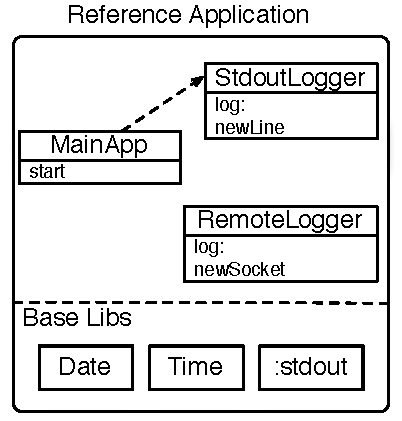
\includegraphics[width=.5\linewidth]{example_reference}
\caption{\small\textbf{Reference application with all code units.}\label{fig:example_reference}}
\end{center}
\end{figure}


\begin{figure*}[ht]
\begin{center}
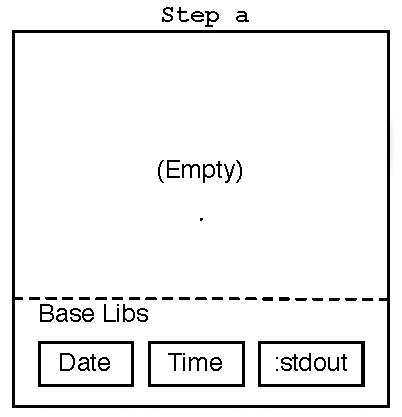
\includegraphics[width=.322\linewidth]{example_before}
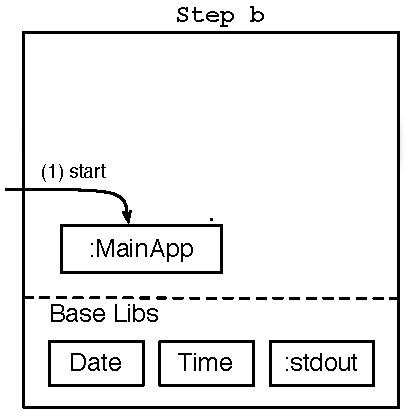
\includegraphics[width=.33\linewidth]{example_starting_point}
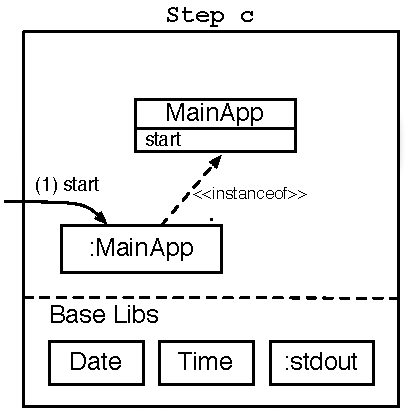
\includegraphics[width=.33\linewidth]{example_dnu_trap_start}
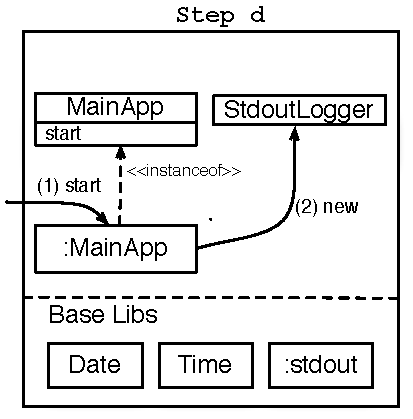
\includegraphics[width=.33\linewidth]{example_shadow_trap}
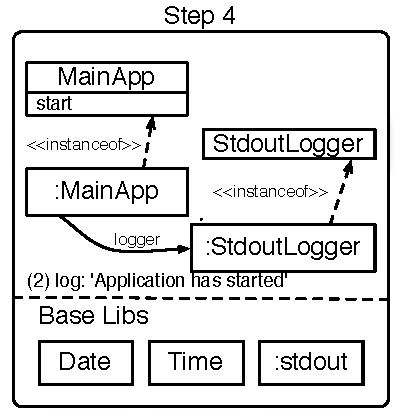
\includegraphics[width=.325\linewidth]{example_dnu_trap}
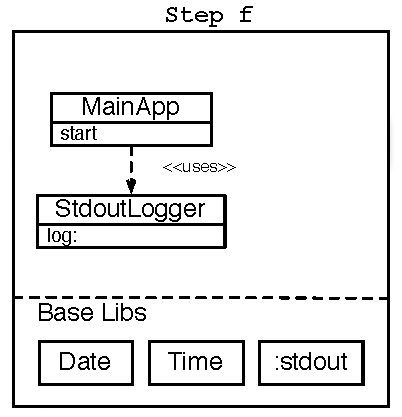
\includegraphics[width=.33\linewidth]{example_finished}
\caption{\small\textbf{The nurtured application at different steps of tailoring.} \label{fig:example_all}}
\end{center}
\end{figure*}

\paragraph{Install the application's entry point} We install into the nurtured application our application's entry point \ie a \ct{MainApp} instance~(\ct{aMainApp}) and a process that will execute the statement \ct{"aMainApp start"}~(cf. Figure~\ref{fig:example_all} Step 1). Note that although we are referencing an instance of the class \ct{MainApp}, the \ct{MainApp} class is not installed yet.

%\begin{figure}[ht]
%\begin{center}
%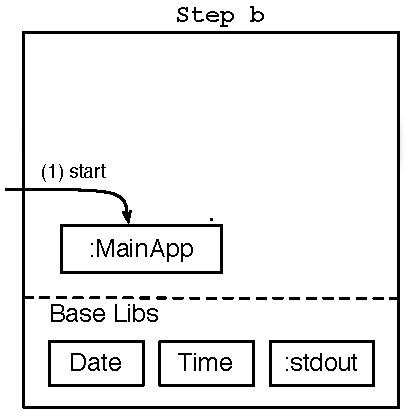
\includegraphics[width=.8\linewidth]{example_starting_point}
%\caption{\textbf{Installing an entry point.} The nurturer installs the entry point of the application and starts its execution sending it the \ct{start} message.\label{fig:example_starting_point}}
%\end{center}
%\end{figure}

When the execution starts, the \ct{mainApp} instance receives the \ct{start} message, and we detect the \ct{MainApp} class and its \ct{start} method as a missing code unit failure. We install these two missing code units~(cf. Figure~\ref{fig:example_all} Step 2) and finally the \ct{MainApp>>start} method is activated and starts running.

%\begin{figure}[ht]
%\begin{center}
%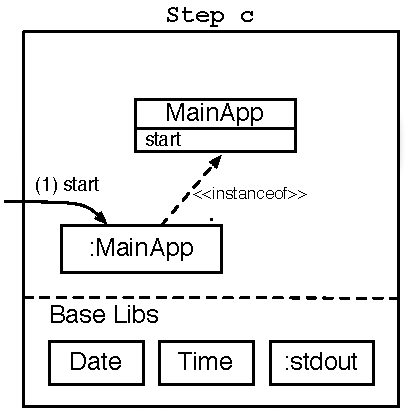
\includegraphics[width=.8\linewidth]{example_dnu_trap_start}
%\caption{\textbf{Activating the entry point.} The nurturer installs the \ct{MainApp} class and the \ct{start} method on demand.\label{fig:example_dnu_trap_start}}
%\end{center}
%\end{figure}

\paragraph{Activating the start method}
The method \ct{start} defined in Figure~\ref{fig:code_example1} is executed, as we can see in Figure~\ref{fig:example_all} Step 2. During the execution of its first statement~(line 2 Figure~\ref{fig:code_example1}) we detect a missing code unit failure: The \ct{StdoutLogger} class does not exist. Thus, before continuing, we install a \ct{StdoutLogger} class with the same shape as its reference counterpart~(cf. Figure~\ref{fig:example_all} Step 3). This class does not contain, however, all the methods nor the meta-data (\eg superclass, package, subclasses) from the reference class since they may not be necessary.

%a \emph{shadow} of the \ct{Formatter} class~(Figure~\ref{fig:example_shadow}).\gp{I don't like the word shadow here, since it does not go with the tailor metaphor} The \ct{Formatter} shadow is a proxy object the tailor will use to know if and when the \ct{Formatter} class is used.

%\begin{figure}[ht]
%\begin{center}
%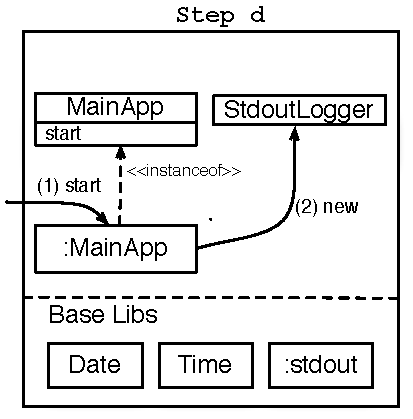
\includegraphics[width=.8\linewidth]{example_shadow_trap}
%\caption{\textbf{Activating the \ct{new} method.} The nurturer installs a the \ct{StdoutLogger} class and sends it the \ct{new} message.\label{fig:example_shadow_trap}}
%\end{center}
%\end{figure}

%Once the \ct{Formatter} shadow is available, the tailor can continue the execution and send the message \ct{new} to the shadow object. At this point, the tailor finds out that the receiver of the \ct{new} message is a shadow object, and thus, it replaces the shadow object by

%Note that copies of classes are treated specially: they contain a method dictionary where methods are installed, but since no instance of \ct{Formatter} received yet a message, its method dictionary is empty.

Once we install the \ct{StdoutLogger} class, we resume the execution. The first statement results into a new \ct{StdoutLogger} instance. Not that the \ct{new} method is not installed because this method is part of the language base library, already available in the seed. 
% The next expression of the \ct{start} method is now ready to be executed.

During the second statement's execution~(line 3 Figure~\ref{fig:code_example1}), we detect a missing code unit failure on the \ct{log:} message~(cf. Figure~\ref{fig:example_all} Step 4): the corresponding method is not installed in the \ct{StdoutLogger} class. We install the method inside the corresponding class and resume the execution. This time the method is found, and the \ct{log:} method is activated.

%\begin{figure*}[ht]
%\begin{center}
%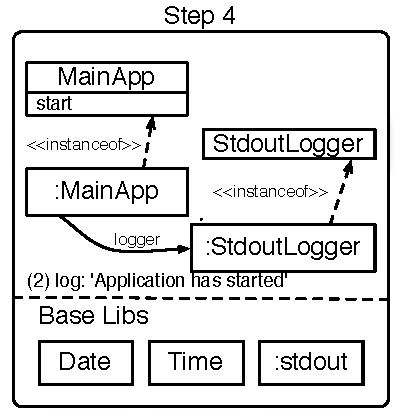
\includegraphics[width=0.65\linewidth]{example_dnu_trap}
%\caption{\textbf{Activating the \ct{log:} method.} The message \ct{log: 'Application has started'} is sent to the \ct{logger} object. \label{fig:example_dnu_trap}}
%\end{center}
%\end{figure*}


Once the \ct{log:} method finishes, the execution returns to the \ct{start} method. There, the third statement~(line 5 Figure~\ref{fig:code_example1}) is executed with no intervention of our technique, since the \ct{log:} method is already available. Figure~\ref{fig:example_all} Step 5 shows the final state of the nurtured application: it contains only the methods and classes that are actually used by the application. Leaf objects used during the process have been garbage collected.

%\begin{figure}[ht]
%\begin{center}
%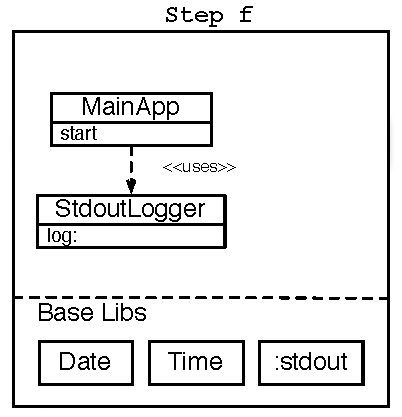
\includegraphics[width=.8\linewidth]{example_finished}
%\caption{\textbf{Final state of the nurtured application.} The nurturing has finished and the resulting application is tailored.\label{fig:example_finished}}
%\end{center}
%\end{figure}

\section{Detecting Missing Code Units}\label{sec:model_detail}


RFG depends on getting notified when a missing code unit failure appears. RFG's algorithm is based on traps to achieve this task, as shown in Algorithm~\ref{alg:tailoring_process}. Traps are placeholders that are installed in the nurtured application in the place of real elements. They are triggered whenever the application tries to access them. In case a trap is triggered, we suspend the nurtured application execution, we install the missing code units replacing their corresponding traps, and finally resume the execution from the moment immediately before the trap was triggered. Traps are installed dynamically in the nurtured application following the information flow of the application \eg when a method \ct{A} is installed some traps are installed inside it to capture possible missing code unit failures it may cause.

We identified the following as the basic traps that are necessary to tailor an application:

\begin{description}
\item[Missing object trap.] A \emph{missing object} trap captures messages sent to objects that do not yet exist inside the nurtured application such as classes. When RFG finds one of these traps, its responsibility is to install the corresponding object. The object installed is a \emph{partial} clone of the original object \ie not all of its state is installed, instead it contains traps to capture the access to its class and fields. When a method refers to a static variable, we install one of this traps for it.

\item[Missing method trap.] A \emph{missing method} trap captures me\-thod invocations whose methods are not defined in the nurtured application yet. When the application execution triggers one of these traps, RFG installs the corresponding method in the class hierarchy of the object. In case of missing classes, RFG installs them too. Missing method traps capture also overridden methods. If an overridden method is not trapped, the method lookup may find a superclass implementation and execute it, resulting into an unexpected behavior. Figure~\ref{fig:need_override} illustrates this problem: the class \ct{B} from the reference application contains an override, while it is not present in the nurtured application. If no trap is placed to capture the override, the method \ct{doSomething} from class \ct{A} would be executed, thus changing the semantics of our application.

\end{description}

\begin{algorithm}[ht]
 %\KwData{this text}
 %\KwResult{how to write algorithm with \LaTeX2e }
 Initialize reference application\;
 Initialize nurturing application with the seed\;
 Install entry point(s)\;
 \While{not finished}{
  run the nurtured application\;
  \If{trap was activated}{
   install missing code units\;
   restart message send;
  }
 }
 \caption{\small An abstract view of the run-fail-grow process \label{alg:tailoring_process}}
\end{algorithm}


\begin{figure}[ht]
\begin{center}
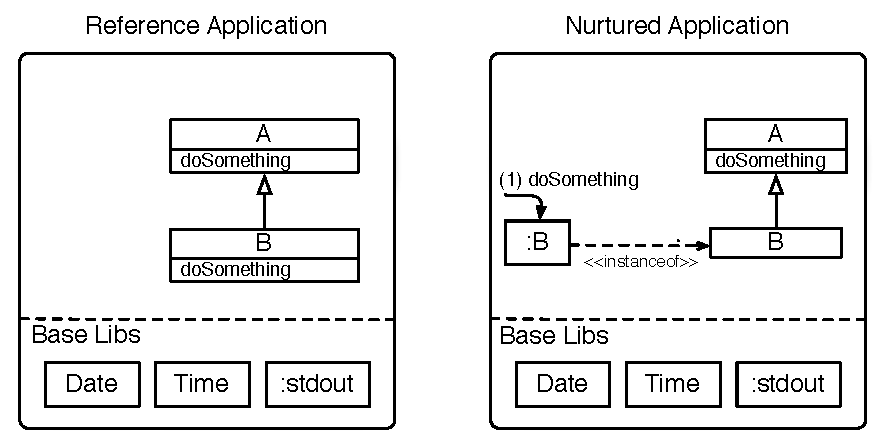
\includegraphics[width=0.7\linewidth]{need_override}
\caption{\small\textbf{The need of overriding traps.} \small Method traps should capture the overridden \ct{doSomething} message-send to avoid the superclass method to be executed wrongly.\label{fig:need_override}}
\end{center}
\end{figure}



\section{Customizing Dead Code Elimination with Seeds}\label{sec:seeds}

The level of tailoring of RFG can be specified using seeds. A seed is a collection of code units whose installation is forced into the nurtured application. These code units are available for the nurtured application and thus, accessing them does not trigger missing code unit failures.

A seed can contain any arbitrary code unit, including package, classes, methods and even already initialized objects. Seeds are useful to cover different tailoring scenarios. Let's take as a first example a smartphone where the base libraries of the language are already available, so they are shared amongst the many applications installed in it. When targeting such a smartphone, base libraries are already present and we do not need to produce an specialized version of them, but specialize only third part libraries and application code. In this case, we use a seed providing the language base libraries. Let's take as a second example a constrained device robot-like which will contain only our application. When targeting this robot as deployment scenario, we want to specialize all the code to deploy including base libraries. In such a case, the seed is empty to allow the RFG algorithm to work on every code unit.

Figure \ref{fig:nurturing_map_model} presents two tailoring maps showing exemplar usages of seeds. Each application contains code units corresponding for the base libraries, third party libraries and application code. In the left the seed covers base and third party libraries, thus RFG applies and selects a subset of the application code units only. In the right, the seed covers only the base libraries, thus RFG applies and select a subset of the code units from the third party libraries and application code.

\begin{figure}[ht]
\begin{center}
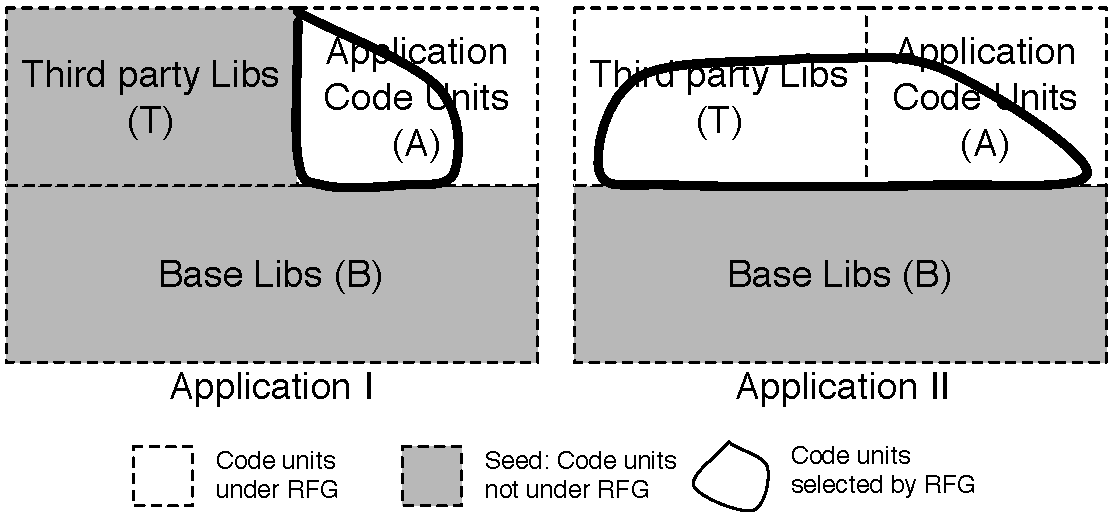
\includegraphics[width=.7\linewidth]{nurture_map}
\caption{\small\textbf{Tailoring Map.} A tailoring map describes which code units of an application are included in the seed~(in gray), which ones are subject to the RFG technique~(in white) and the amount of them that are finally selected~(within the thick area).
\label{fig:nurturing_map_model}}
\end{center}
\end{figure}


%============================================================================
\section{Tornado: RFG in \Vtt} \label{sec:rfg_implementation}

We implemented our RFG technique as a tool called \emph{Tornado}. Tornado is implemented using \Vtt, to tailor applications written in the Pharo programming language.
%Pharo is a reflective and dynamic programming language inspired from Smalltalk.
Tornado's architecture combines \Vtt~(cf. \chapref{vtt}) and Ghost proxies~(cf. Section \ref{sec:proxies}) illustrated in Figure \ref{fig:tornado_code units}. The nurtured application is hosted inside an object space  Tornado's hypervisor runs and monitors the nurtured application. It installs traps on the nurtured application as Ghost proxies, and use the object space interface to query and install code units it. Following, we detail how we fulfilled each of RFG's requirements in our solution:

\begin{figure}[ht]
\begin{center}
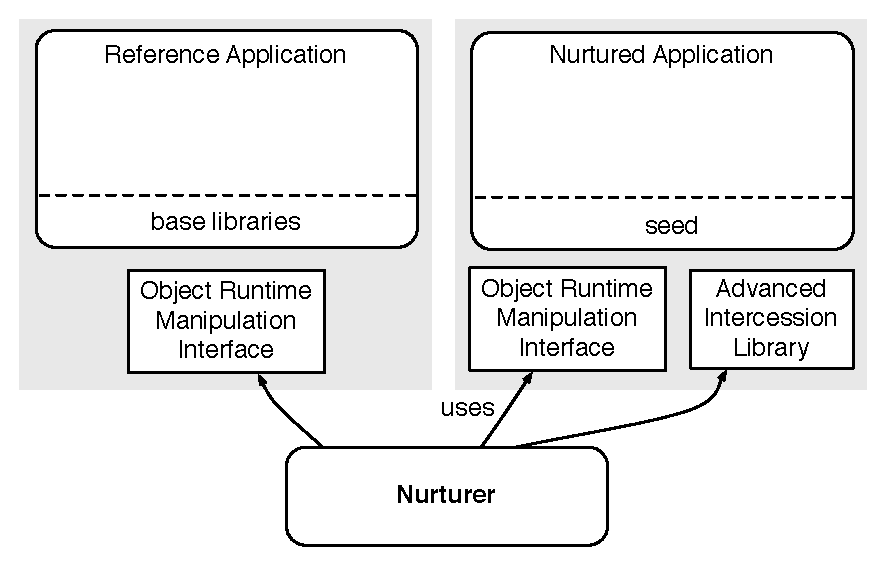
\includegraphics[width=0.8\linewidth]{tornado_components2}
\caption{\small\textbf{Tornado's architecture overview.} Tornado controls both the reference and nurtured applications through Oz. Traps are installed into the nurtured application with the Ghost library.\label{fig:tornado_code units}}
\end{center}
\end{figure}

\begin{description}
\item[Execution cycles.] We use \Vtt execution cycles to monitor and control the execution of a nurtured application. When a cycle is finished the Tornado hypervisor checks if the virtualized runtime is suspended on a trap. In such case, it installs the corresponding code unit and resumes the execution with another cycle.

\item[Advanced proxies.] Pharo's libraries includes Ghost~\cite{Mart11a}, an advanced proxy implementation. Ghost allows one to capture all kind of message sends, intercept particular method executions, and even to proxy classes and special objects. We use the Ghost model to implement execution traps.

\item[Object space runtime manipulation.] An object space provide already with operations to query and install the classes and methods in the virtualized runtime.

\end{description}

\subsection{Execution Traps with Ghost Proxies} \label{sec:proxies}

Implementing execution traps such as the ones described in Section~\ref{sec:model_detail} requires powerful intercession support. Traps must capture \emph{all} message sends to objects provided by the application runtime as well as the application objects, including classes~(for example for the case of class messages or static methods). They must capture \emph{self} and \emph{super} message sends, as well as overrides and particular method invocations.

To achieve this, we implemented a set of proxies following the Ghost model~\cite{Mart11a}~(similar to JavaScript proxies~\cite{Vanc10a}). Ghost proposes a low-memory footprint, general purpose proxy implementation for the Smalltalk language supporting the creation of proxies for normal objects as well as classes and methods. 
% These proxies allow the interception of all message sends.
% When a Ghost proxy captures an invocation, it triggers the behavior of a \emph{handler}. 
% The Ghost proxy library provides already several kinds of handlers including for example message forwarding or logging.
Using Ghost proxies we are able to detect all situations corresponding to our traps.
Ghost proxies represent missing objects, classes and methods. When a proxy is accessed, Tornado replaces it by its corresponding real object.
Tornado correctly respect identity by using a table relating each proxy to the code unit or object it represents in the reference application.
%Ghost proxies capture all messages.
Additionally, each proxy is attached to a \emph{handler} that may perform some action when the proxy receives a message.
We use proxy handlers to perform the right action for each trap.
We discuss below the different kinds of proxies and handlers we use and how they support RFG.

\begin{description}
\item[Missing object trap.] This trap is implemented as a proxy taking the place of a normal object. This trap is triggered when the proxy receives a message.
Its handler replaces the proxy by a \emph{partial} copy of the original object from the reference application.
The copy is created, and all references to the proxy are replaced by references to this new object, which is achieved through the \ct{become:} facility of the Pharo language that dynamically swaps object references.
Each field and the class of this new installed object are installed as new missing object traps.

\item[Missing method trap.]  We implemented the missing method trap in Tornado as a class proxy located at the top of the class hierarchy. Whenever a message is sent to an object, the VM looks up the method in the object's class hierarchy. This trap is triggered whether a message arrives to the top of the hierarchy, meaning that there was no method for it in the hierarchy. When triggered, the handler installs the classes part of the hierarchy of this method and the missing method in its corresponding class. If no method is found to install, Tornado sends the \ct{doesNotUnderstand:} message~(an equivalent to \eg Ruby's \ct{method\_missing} and Python's \ct{\_\_getattr\_\_}) to honor the dynamic semantics of Pharo.

\item[Missing override trap.] We implemented missing override traps in Tornado using method proxies. Method proxies are placed in the method dictionaries of classes containing overriden methods, taking the place of the original method.  When Tornado installs a class into the nurtured application that contains overridden methods in the reference object space, it installs into this class a method proxy for each of its overridden methods. This trap is triggered whenever the method proxy it is about to be executed. The handler of this trap compiles a new method with the same source as the corresponding method from the reference application and installs it inside the nurtured object space.

\item[Primitive methods trap.] Primitive method traps are implementation specific related to the Pharo language. Pharo's primitive operations such as number arithmetic are implemented through primitive methods. Primitive methods are implemented in the Virtual Machine and do often access directly the fields of its receiver and arguments by forging references and manipulating directly the memory, bypassing our traps. Thus, we face an issue when a \emph{missing object trap} proxy is the argument of such a method: the VM can modify this proxy without activating the trap. Primitive method traps are method proxies that decorate Pharo's primitive methods. When they are triggered because one of these methods is about to be executed this trap's handler triggers each of the missing object traps received as arguments, if any. In this way, Tornado forces the installation of the arguments and the primitive is executed with actual objects instead of proxies, as expected.

\end{description}

% \subsection{Traps and Proxies}\label{sec:traps}
% Tornado traps notify the nurturer when some object is missing. In such case, the tailor installs the missing object and continues the execution from the point where it was trapped. Traps are implemented in Tornado through Ghost like proxies. Each trap in tornado is a Ghost proxy. Tornado implements a custom interception handler: every time a trap is activated, the object space where the trap is located gets paused and the control is returned to the tailor to treat the trap. Following, we explain each of the traps implementations and how they are treated by the tailor:
% 
% \begin{description}
% \item[Not-installed trap.] A trap for an object or class not yet installed in the system is a simple proxy. If the proxy receives a message, the tailor installs the object the proxy represents and replaces the proxy by the new object. If the new object has fields, these fields will be propagated as proxies or installed depending on its particular mapping~(cf. section~\ref{sec:mappings}). In our particular implementation, the replacement of the proxy by its new counterpart is done through the \ct{become:} facility of the Pharo language that allows pointer swapping.
% \item[Does not understand trap.] We implemented the does not understand trap in tornado as a class proxy situated on the top of the class hierarchy. Whenever a message is sent to an object, the method lookup mechanism searches a method with the same firm in the object's class hierarchy, starting from the object's class up to the top. Our does not understand trap captures whether a message arrives to the top of the hierarchy, meaning that there was no method for it in the hierarchy. When this trap is activated, the tailor looks in the model application for the method to install, installs it in the nurtured application and finally restarts the execution from the call-site that activated the trap.
% 
% \item[Override trap.] We implemented override traps in tornado using method proxies. Method proxies are activated whenever the proxified method is about to be executed. When Tornado installs a class that contains overridden methods in the reference object space, it also installs into it one method proxy for each of its overridden methods. In such a way, the method lookup mechanism finds the overridden traps and returns the control to the tailor. In turn, the tailor installs the method corresponding to the trap and restarts the execution from the call-site that activated the trap.
% 
% \item[Primitive methods trap.] \gp{il faut l'ecrire}
% 
% \end{description}
% 
% \gp{Traps are placed in the tailoring application so they get activated only when the special cases are given. They do not represent a penalty on runtime during the tailoring process.}
% 
% Note that every time a trap is captured and treated, restarting the execution must handle correctly self and super message-sends\footnote{A super message-send starts the method lookup from the superclass of the class where the actual method in execution is located, instead of the class of the message receiver}. Thus, Tornado always restarts the execution respecting the call-site and the class where the method lookup mechanism started to maintain the program's semantics, regardless the kind of trap that was activated.


\subsection{Object Installation and Propagation Rules} \label{sec:mappings}

As we explained before, Tornado installs all objects inside the nurtured application on demand, as \emph{partial copies}, \ie the objects referenced by the original object will not be copied along with it by default, but traps are placed instead of them. %That is, no object, class or method is installed unless it is needed by the application to run. The need for installing some element is detected by means of traps~(cf. Section~\ref{sec:model_detail}).
%The tailored application contains during the tailored process two kind of objects: application objects that are copies of the model application objects, and proxy objects representing traps.
When Tornado installs an object inside the nurtured application, this new object has the same format and size as its original counterpart. \emph{Propagation rules} determine how each of the object's fields are propagated on installation. Tornado provides the following propagation rules to customize installation:

\begin{description}
\item[Missing object trap.] This is the \emph{default propagation rule} and end user applications can usually be tailored with just them. This propagation rule installs a missing object trap in each field of the object that is being installed.
\item[Materialization.] This propagation rule forces the installation of the object referenced by the field. This is used for those cases where some structure should be guaranteed to the Virtual Machine \eg the objects referenced by the first three fields of a class~(superclass, format and method dictionary) cannot be proxified because they are used by the VM for the method lookup. The same happens with other objects reifying low level concepts such as activation records or semaphores.
\item[Swapping.] This propagation rule forces the reference of the object installed be swapped to another object's reference. The usual use case of this rule is replacing some object reference by \ct{nil}, and so, to force lazy initializations.
\end{description}

% Figure \ref{fig:character_mapping} shows an example of the mapping of the \ct{Character} class which forces the materialization of the character and digit tables class variables.
%
%\begin{figure}[ht]
%\small
%\begin{code}
%Character >> tornadoMappingFor: aTornado
%	^ (super tornadoMappingFor: aTornado)
%			mapClassPoolWith: { 
%				#CharacterTable -> ToMaterializationPropagationStrategy new.
%				#DigitValues -> ToMaterializationPropagationStrategy new
%			}; yourself
%\end{code}
%\caption{\small\textbf{Mapping for class \ct{Character}.} Mapping forcing the installation of the character and digit tables needed by the VM. \label{fig:character_mapping}}
%\end{figure}

\subsection{Object Identity and Proxies}

Tornado takes care of the identity of objects with an identity table. The identity table is important because Tornado works at the object granularity. Due to the inherent graph nature of object-oriented programs, an object being installed may reference another object that is already installed inside the nurtured application.
Identity is an important concern in the presence of proxies. Tornado guarantees that identity checks inside a program~(\eg comparison through \ct{==}) always preserve object identity by following the following invariant: 

\begin{center}\emph{An object and its proxy do not exist concurrently in the nurtured application.}\end{center}

That is, the nurtured application contains either an object, either the proxy trap that represents its absence, but not both at the same point in time. When the proxy is replaced by the actual object's copy, all references to the proxy are swapped to references to the new object. The proxy is no longer referenced and thus, garbage collected. This invariant guarantees that identity checks in a program that should be \ct{true} are indeed be \ct{true}. Either the compared references point both to the same proxy, or both to the same \emph{partial} copy.

\subsection{Implementing Seeds in Tornado}

Tornado's seeds specify the level of tailoring. The seeds are in charge of initializing the nurtured application's virtualized runtime with the elements we want to ensure on it. Our current prototype supports two ways of describing and building seeds: 

\begin{description}
\item[Loading an already existing memory snapshot.] The nurtured application's object space is initialized by loading an already existing snapshot or image~(\ie this is an image in the same sense as Smalltalk or Lisp). This technique consists in using a memory dump from an object heap containing all the classes and objects desired in the seed. This memory snapshot should follow Pharo's object format. 
\item[Creating all seed code units from scratch.] The nurtured application's object space is initialized with objects built from scratch. This technique uses a bootstrapping process as described in \chapref{bootstrapping}.
\end{description}

%Note that a seed can indeed contain any arbitrary code units and objects. They are not restricted to have only base or third party libraries. The selection or extraction of what is included as part of a seed is application dependent and orthogonal to the run-fail-grow process. We show an example of it in Section \ref{sec:results}.

\subsection{Preparing the Application for Deployment}\label{sec:deploy}

Once Tornado is stopped, the nurtured application contains all the code units needed to run. Tornado procceeds to prepare the application for deployment \ie it removes all trap leftovers and extracts the nurtured application. Tornado identifies the traps by the presence of proxies and replaces the references to those proxies by references to another object, defaulting to the \ct{nil} object. Proxy objects do not then represent a drawback in space consumption because they are garbage collected. Once the traps are removed, the nurtured application keeps no dependencies to Tornado nor its infrastructure. Thus, the application can run outside the Oz infrastructure with no performance penalties.

Finally, Tornado extracts the application code units using one of two different techniques: (a) the creation of a snapshot file containing all code units and already initialized objects; or (b) build a static description of the application containing the code for all classes and methods that should be part of it.

\section{Conclusion and Summary}

In this chapter we presented a run-fail-grow~(RFG) approach for application tailoring. RFG tailors an application by starting it and initializing it with a seed that contains the minimal set of code units we want to ensure. Then, we install and execute the application's entry points. As the application executes, missing code units are found and installed on demand, ensuring that only the needed code units are introduced. By following the runtime execution, it supports dynamic features such as reflection and meta-programming.

We implemented RFG in a tool called Tornado based in \Vtt. With \Vtt, we are able to monitor the nurtured application's execution using the execution cycles. Mirrors allows us to easily install required code and restart the execution as it is needed.

\chapter{Validation}

\introduction

%\section{Experiments and Results}\label{sec:results}
%
%\subsection{Experiment's Methodology}
We evaluate Tornado by conducting five experiments that tailor different Pharo applications, with increasing requirements~(Section \ref{sec:rfg_experiments}). We chose our experiments under the objectives of (a) understand how minimal are the applications we can tailor, (b) explore how successfully we address the challenges we stated in Section \ref{sec:challenges} and (c) exercise those cases that push to the limit the interaction between the language and the VM. Our experiment methodology consists in the following steps:

\begin{enumerate}
\item \textbf{Setting up a seed for the application.} Most of our experiments use what we already called an \emph{empty seed}. This seed is, however, not completely empty. The empty seed we used contains some minimal infrastructural objects that are needed for language-VM interaction, and is therefore 10KB large. Our last experiment, the largest one, uses both this empty seed and an additional seed containing the base libraries. 
\item \textbf{Preparing the application entry points.} This step consists in the installation of the one or more processes that will run our application.
\item \textbf{Run the application.} The application is run, its threads executed. In particular in our last experiment~(an interactive web application), we interact with our application through a web browser. 
\item \textbf{Stop and extract the application.} Once the tailoring process finishes, we stop Tornado and extract the resulting application by making a snapshot of it in a Pharo image file. We test the generated snapshots to verify they work properly, either by using the application or debugging them when they involve no I/O. We evaluate the behavior of the tailored application under the assumption that only the features we used during the tailoring should work.
\item \textbf{Perform measurements.} Finally, we measure the size of the generated snapshots files and compare them against two different Pharo distributions prepared for production~(cf. Section \ref{sec:results_discussion}).
\end{enumerate}

Additionally, we present an evaluation of Tornado according to the evaluation criteria stated in \chapref{state_virtualization}. Our evaluation includes a comparison with the already presented related work on application tailoring~(Section~\ref{sec:rfg_evaluation}).
Finally, we discuss some aspects and trade-offs of the run-fail-grow approach and our implementation~(Section~\ref{sec:discussion}).

\section{Experiments}\label{sec:rfg_experiments}

\subsection*{Experiment I: Adding Two Numbers}

The smallest~(in terms of size) interesting program to tailor is adding two numbers, without the involvement of any I/O \ie an application just executing the \ct{"2 + 3"} statement as entry point. Tailoring this program is challenging because it stresses the infrastructure by installing only the minimal elements an application needs to run. It makes evident how small a tailored application can be. Additionally, it is interesting since it makes use of the following features of the Pharo language and infrastructure:

\begin{description}
\item[Immediate objects.] Immediate objects are objects encoded in the object reference instead of being allocated in the heap. Immediate objects do not contain a reference to their class in the object header, as there is no object header. Instead, the object reference where the object is encoded contains a bit tag that the VM uses to identify the immediate object. This means that the Pharo VM must acknowledge the immediate object classes~(or their proxies) in order to send messages to these immediate objects. In this experiment we use immediate small integers, instances of \ct{SmallInteger}.
\item[Special selectors.] The method selector \ct{+} is a special selector for the Pharo VM. Special selectors are optimized as they are broadly used messages, for example for arithmetics. First, they are implemented as special bytecodes to avoid method lookup. If the special bytecode cannot be executed because some VM assertions are not valid~(\eg class and object format assumptions), the VM performs the default method lookup. In this experiment the VM should take care of small integer arithmetic \ie it should fulfill all VM assumptions and not perform a method lookup; Tornado should install no extra methods nor classes.
\end{description}

\subsection*{Experiment II: Factorial of a little number}

The following experiment in incremental complexity is the factorial of a small number, again without the involvement of any I/O \ie an application executing the \ct{"10 factorial"} statement as its entry point. Factorial uses arithmetic as the latter experiment~(sums and multiplications), while it also adds the following interesting cases:

\begin{description}
\item[Method lookup.] The \ct{factorial} message is sent to a small integer but not optimized as it is not a special selector. Thus, the VM look ups the corresponding method up in its class hierarchy. The method \ct{factorial} is defined in its superclass~(\ct{Integer}).
\item[Recursion.] The factorial implementation in Pharo base libraries is recursive. Additionally, this recursion activates the \ct{factorial} method many times, creating many activation records in the VM. Activation records are reified lazily whenever it is accessed reflectively, or the stack depth is deeper than the maximum supported.
\end{description}

\subsection*{Experiment III: Factorial of a large number}

Following, we experimented with an application whose entry point was the \ct{"100 factorial"} statement. This application does not either make use of any I/O. The factorial of a large integer creates eventually integers that exceed 32 bits, and thus, do not fit as immediate small integers. This experiment adds the following interesting cases:
\begin{description}
\item[Large integers.] Large integers in Pharo are represented, in contrast to immediate small integers, as objects allocated in the heap with their own object header and arbitrary length. Large integers are created automatically by the VM when the result of some integer calculation produces a number that overflows 31 bits. That is, the LargeInteger class (or its proxy) should be available to the VM in order to instantiate the correct object.  Additionally, large integers implement their arithmetic methods by calling primitives from external plugins~(the large integers plugin).
\item[Polymorphism.] The introduction of large integers introduces also \emph{polymorphism} between them and the immediate small integers. They share the same class hierarchy~(\ct{Integer} is the superclass of \ct{SmallInteger} and \ct{LargePositiveInteger}), being the method \ct{factorial} implemented in the superclass and having each of the subclasses their own implementation of the arithmetic methods for adding and multiplying.
\end{description}

\subsection*{Experiment IV: Reflective invocations} \label{sec:results_helloworld}

The fourth experiment introduces reflective invocations. Figure \ref{fig:reflective_invocations} introduces the code we used for this experiment. The \ct{User} class in our example has two fields (\ct{name} and \ct{age}), and four methods. Two of these methods (\ct{age} and \ct{name}) return directly the field with the same name, the method \ct{hasWritePermissions} is annotated with the \ct{property} annotation (a pragma in Pharo's terminology) and the method \ct{isMinor} is a normal method. We introduce also \ct{PropertyExtractor} class with the responsibility of returning the name of those methods that are properties of an object \ie all methods that only return a field, and all those methods annotated with the \ct{property} annotation. The statement we introduced as the entry point for this experiment is \ct{"PropertyExtractor new extractPropertiesFrom: User new"}.

\begin{figure}[ht]
\small
\begin{code}
Object subclass: #User
	instanceVariableNames: 'name age'.

User>>age
	^ age

User>>hasWritePermissions
	<property>
	^ true

User>>name
	^ name

PropertyExtractor>>extractPropertiesFrom: anObject
	^ anObject class methods
		select: [ :each | each isReturnField
			or: [ each pragmas anySatisfy: [ :pragma | pragma keyword = #property ] ] ]
		thenCollect: [ :each | each selector ]

\end{code}
\caption{\small \textbf{Code of the reflective invocations experiment.} The \ct{PropertyExtractor} class does the reflective invocations, the \ct{User} is the class we will be reflecting on.\label{fig:reflective_invocations}}
\end{figure}

This experiment evaluates how do we handle the reflective abilities of Tornado's RFG. The \ct{PropertyExtractor} queries the methods from the \ct{User} class, that are included as part of the tailored application~(since they receive the messages \ct{isReturnField} and \ct{pragmas}). These reflective invocations include: (a) access to an object's class, (b) access class methods and (c) query those methods to know if they correspond to the criteria of the \ct{PropertyExtractor}.

\subsection*{Experiment V: Adding I/O} \label{sec:results_helloworld}

A fifth experiment introduces I/O to each of the previous experiments, adding a statement printing to the standard output the obtained results. Figure~\ref{fig:hello_world_entry_point} shows the code from our entry point in the case of summing up two numbers. The entry points for the other experiments have the same structure, differing only on the expression that is printed~(the \ct{"1+2"} expression in this case). Notice that the \ct{FileStream} class needs to be initialized before the proper printing into the stdout stream because the code needed for class initialization is not installed by default in the empty seed.

\begin{figure}[ht]
\small
\begin{code}
FileStream startUp: true.
FileStream stdout 
	nextPutAll: (1 + 2) asString;
	crlf.
\end{code}
\caption{\small \textbf{Entry point of the experiment that sums two numbers and prints the result in the standard output stream.}\label{fig:hello_world_entry_point}}
\end{figure}

In this experiment, besides testing the proper usage of I/O streams such as the standard output stream, we evaluate the ability of Tornado to handle \textbf{platform identification}. The \ct{stdout} stream initialization for Pharo is done by the File package written in Pharo, and it depends on which is the current operating system. This experiment shows that Tornado prepares tailored versions of applications to run on a single operating system or platform.

\subsection*{Experiment VI: Seaside Web Application}



Our last experiment consists is tailoring a web application using Seaside application framework~\cite{Duca07a}. Seaside is a web application framework featuring continuations thanks to stack reification. We configured it with its default values, without making any customizations. The web application under tailoring has a single webpage that allows one to send requests to the web server to increase or decrease a counter. This experience shows that Tornado works in presence of \textbf{threading}. The Seaside application framework makes use of Pharo processes. One process listens incoming connections and opens new processes to handle requests. Seaside uses semaphores to synchronize processes and wait for incoming data from sockets.

For this case, we proceeded to do two different experiences, with two different seeds. We first used the empty seed~(\emph{Seaside Web Application A}), as in the previous experiments, and then used a seed containing all Pharo base libraries~(\emph{Seaside Web Application B}). For reasons of space, the details of how the entry points are initialized for these both seeds can be found in our technical report~\cite{Poli14a}.

\section{Results} \label{sec:results_discussion}

We gathered our experiments' results into Table \ref{tb:results}. This table shows:
\begin{description}
\item[Experiment.] The name of the experiment under evaluation, followed by our measurements.
\item[Reference Application.] The size of the reference application containing all of its code units, in KB. We present in here two different sizes: the size of an experimental shrunk version of the Pharo distribution called \emph{PharoKernel}, which was developed independently from us by Pavel Krivanek; and between parenthesis the size of the official Pharo distribution prepared for production: Pharo allows one to prepare a snapshot for production. This option cleans some caches and removes some well known objects and classes from the system, thus, freeing space.
\item[Seed.] The size in KB of the chosen seed for the experiment.
\item[Nurtured Application.] The final size of the nurtured application once Tornado finishes its process and the application is extracted.
\item[Saved.] The percentage of space saved using the smallest reference application size. We chose the smallest reference application to avoid biased results in our favor. We calculated this percentage using the following equation:

\begin{equation*}
saved = 100 - \frac{100*(nurtured - seed)}{reference - seed}
\end{equation*}

\begin{table}[ht]
 	\centering
 	\begin{tabular}{lccccc}
		\toprule
			Experiment
 			& \textbf{Reference App}
			& \textbf{Seed}
			& \textbf{Nurtured}
			& \textbf{Installed}
			& \textbf{Saved(\%)}\\
			
 			& \textbf{\emph{Shrunk(Prod.)}}
			& \textbf{Size}
			& \textbf{App}
			& \textbf{Code}
			& \textbf{}\\
		\toprule
		Sum Two
 			&  3799 (12873) & 10 & 11 & 1 & \textbf{99.97\%}\\
		Numbers (I)
 			& &&&&\\
		\midrule
		Fact 10 (II)
 			& 3799 (12873) & 10 & 15 & 5 & \textbf{99.87\%}\\
		\midrule
		Fact 100 (III)
 			& 3799 (12873) & 10 & 18 & 8 & \textbf{99.79\%}\\
		\midrule
		Reflective
 			& 3799 (12873) & 10 & 32 & 22 & \textbf{99.42\%}\\
		App (IV)&&&&&\\
		\midrule
		(I) + I/O
 			& 3799 (12873) & 10 & 81 & 71 & \textbf{98.13\%}\\
		\midrule
		(II) + I/O
 			& 3799 (12873) & 10 & 82 & 72 & \textbf{98.10\%}\\
		\midrule
		(III) + I/O
 			& 3799 (12873) & 10 & 89 & 79 & \textbf{97.92\%}\\
		\midrule
		(IV) + I/O
 			& 3799 (12873) & 10 & 95 & 85 & \textbf{97.76\%}\\
		\midrule
		Seaside Web
 			& 20254 (17250) & 10 & 573 & 563 & \textbf{96.73\%}\\
		App A&&&&&\\
		\midrule
		Seaside Web
 			& 20254 (17250) & 12872 & 13090 & 218 & \textbf{95.02\%}\\
		App B&&&&&\\
		\bottomrule
 	\end{tabular}
 	\caption{\small\textbf{Results of the tailored experiments.} Sizes are displayed in KB. The percentage of saved space does not take into account the seed, as it is not subject of Tornado and it is shared by both the reference and nurtured application.}
 	\label{tb:results}
 \end{table}


Note that we subtract the size of the seed from both the nurtured and reference applications sizes, since the seed is shared between both. That way, we compare only those parts of the application that were subject of the RFG algorithm.

\end{description}

 \begin{table}[ht]
 	\centering
 	\begin{tabular}{lc}
			\toprule
			\textbf{Component}
 			& \textbf{Size~(KB)}\\
		\toprule
		Pharo Base Libraries & 12872\\\midrule
		Seaside Application Framework Libraries & 4378\\\midrule
		Seaside Web App & 47\\\midrule
		Reflective Invocations App & 104\\\bottomrule
 	\end{tabular}
 	\caption{\small\textbf{Component sizes in our experiments. Size presented in KB.} \label{tb:tailored_components}}
 	\label{tb:basic_sizes}
 \end{table}

Table \ref{tb:tailored_components} shows the size in KB of the code units from we used in our experiments. This table details the size of the Pharo base libraries, third party libraries such as Seaside and our particular experiments, which aid in the understanding of the results. We obtained this sizes by measuring the size of the code units once loaded in memory.

\subsection{Discussion of Results}
Our experiments show that Tornado aggressively reduces the size of code units required for an application. Our examples save from 95\% to 99\% of space, compared with their reference application~(which contains all base libraries and third party libraries in case of Seaside). Our first three experiments (the sum of two numbers, and the factorial of 10 and 100) show that Tornado succeeds to create minimal deployment versions of our applications, having into account that our seed forces a minimal of 10KB in each of them. The reflective application is indeed also minimal, but bigger than the other three, as Tornado installs inside the nurtured application (a) all the code that is accessed by reflection and (b) code from the collections package to iterate the methods of a class.

We detect a notorious grow in size when adding I/O to our experiments, which varies from 63KB to 71KB extra. According to the list of installed code units, we identity a problem in the design of the I/O streams library from Pharo: a set of character tables meant for character encoding and conversion are initialized, even if not all of them are later on used by the application. This problem shows that this part of Pharo base libraries should be rethought.

The Seaside experiments show that Tornado can be used in a complex setting such as a web application that runs a web server, while still achieving good results. It is interesting to note, from the comparison of both experiments, that more of half of the size of the final nurtured application in \emph{Seaside Web Application A} seems to be in the base libraries, as the amount of installed code is reduced when introducing the base libraries seed.

\subsection{Comparison with a Dedicated Platform}

To have a broader view of our results, we compare them to MicroSqueak~\cite{Malo11a}. MicroSqueak is a dedicated platform that runs on the Pharo platform \ie a specialized platform containing an alternative implementation of base libraries, as Java Micro Edition~(J2ME)~\cite{JavaME} is for Java. MicroSqueak was designed with the explicit goal to be the smallest practical Squeak kernel. It contains a total of 49 classes with a reduced set of methods. It offers a minimal core of the language, a basic collection library and basic file IO support. MicroSqueak presents a minimal memory footprint of 80KB, when we build an application that performs no computation.

On one side, Tornado ensures smaller memory footprints when working on small applications. On the other side, MicroSqueak presents crucial differences with Pharo base libraries: it does not provide the same libraries~(\eg it does not contain socket support) and it does not ensure the same API of those libraries that it contains. Thus, applications such as the one in our Seaside experiment cannot run on top of MicroSqueak without a dedicated version of the Seaside framework.

\section{Evaluation of Tornado}\label{sec:rfg_evaluation}

We start this section evaluating Tornado according to the criteria we presented in \chapref{state_tailoring}, so we can in the following sections discuss it and compare it with other approaches. Table~\ref{tb:comparison} shows an overview of the criteria presented in \chapref{state_tailoring} and their possible values to evaluate tailoring solutions.
In this section we focus on the evaluation of Tornado that is summarized in the latest column of Table~\ref{tb:comparison}.

\begin{table}[ht]
 	\centering
 	\begin{tabular}{cccccc}
	
\toprule
 			& \textbf{Dedicated}
 			& \textbf{Static}
			& \textbf{Hybrid}
 			& \textbf{Dynamic}
			& \textbf{Tornado}  \\
 			& \textbf{platforms}
 			& \textbf{Analysis}
			& \textbf{Analysis}
 			& \textbf{Analysis} &\\
 \toprule

		Base Libraries
 			& + & + & + & + & \textbf{+}\\
		\midrule
		Third-Party
		& & & & \\Libraries
 			& - & + & + & + & \textbf{+}\\
		\midrule
		Legacy Code
 			& - & + & + & \textasciitilde  & \textbf{+}\\
		\midrule
		Reflection Support
 			& + & - & - & +  & \textbf{+}\\
		\midrule
		General Purpose
			& & & & \\
		Infrastructure
 			& + & - & - & \textasciitilde   & \textbf{+}\\
		\midrule
		Configurability
 			& - & - & - & \textasciitilde    & \textbf{+}\\
		\midrule
		Dynamic typing
 			& + & - & - & +  & \textbf{+}\\
		\midrule
		Minimality
 			& - & + & + & \textasciitilde  & \textbf{+}\\
		\midrule
		Completeness
 			& + & - & - & \textasciitilde  & \textbf{-}\\
\bottomrule
 	\end{tabular}
	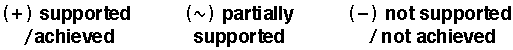
\includegraphics[width=.7\linewidth]{runtime_manipulation_criteria_overview}
 	\caption{Evaluation criteria applied to related work on deployment code unit tailoring techniques}
 	\label{tb:comparison}
 \end{table}

Tornado's model and implementation show themselves as a complete solution in the area of application tailoring. It tailors code units written by the application's developer as well as those from the base language and third-party libraries. There is no special code for managing such cases since Tornado's infrastructure allows the inspection of loaded classes, regardless their origin. This approach, based on runtime execution, offers two main advantages: (a) it does not require modifications in the nurtured application's code allowing its usage on legacy code and libraries in a transparent way, and (b) it supports reflection naturally since the code exercised during the tailoring is the same that will be executed once deployed.

Tornado requires a dedicated infrastructure only during the tailoring: tools to monitor and manipulate the tailoring application. However, once the tailoring is finished and the application reaches a stable point, Tornado extracts and prepares the application to run in the deployment-ready unmodified infrastructure.

Finally, Tornado is a flexible solution in the sense that it allows one to configure the level of tailoring by means of a seed. The seed contains a pre-selection of code units available in the tailoring application before the tailoring starts. In such a way, we can use the seed to specify whether, for example, the base or third-party libraries should be tailored or not.

\section{Discussions on the run-fail-grow approach} \label{sec:discussion}

\subsection{Ensuring Completeness} \label{section:safety}

Dead code elimination techniques do never ensure completeness by themselves. Static approaches cannot efficiently predict the need of those elements used by reflection, or configured in external files/resources. Dynamic approaches depend on the code coverage of the application during runtime, \ie if the parts of the application that are not used will be not available afterwards. Hybrid approaches share both weaknesses. Orthogonal to the dead code elimination techniques, two complementary mechanisms are used by existing solutions to guarantee \emph{completeness} and avoid runtime errors due to missing code.

\begin{description}
\item[Lazy Loading.] JUCE~\cite{Popa04a,Teod01a} and SlimVM~\cite{Kers09a, Wagn11a}, as well as Tornado, load missing code from remote servers on demand, Marea\cite{Mart12a} implements application-level virtual memory with lazy loading of unloaded unused objects. These different solutions differ on their lazy loading approaches by the granularity they use. JUCE loads code with a method granularity to control memory consumption. SlimVM uses as its main loading granularity, a \emph{basic block} granularity, but they can work at the class and method level also. Marea uses an object-cluster granularity. It loads object graphs containing not only classes but also individual objects, which were unloaded to reduce the application's memory footprint.
\item[Remote Invocations.] OLIE~\cite{Gu03a} uses remote invocations to invoke methods from those objects that where offloaded and migrated to other devices. This approach may introduce several latency problems due to network communications. OLIE tries to minimize it by offloading those elements that degrade less the performance of the system. For that, it takes at runtime object and bandwidth usage statistics.
\end{description}

\subsection{Maximizing the Effectiveness of Run-fail-grow}\label{sec:maximize_effectiveness}

Dynamic techniques, in particular Tornado, depend on the coverage of the application to ensure the code is loaded and available for execution. Application coverage must ensure that every code unit that is interesting to be deployed is covered, including special and boundary cases as well as the straightforward cases. We can enforce the coverage and installation of code with several techniques. 

\begin{description}
\item[Manual Testing.] Manual testing provides a simple but inefficient way to cover an application's code. Its main benefit is that the code units selection is based on user interactions. Its main drawback is the possibility of human omission during the testing, which impacts directly the detection of used code. 
\item[Automated Testing.] Automated testing counters the human omissions by adding repeatability in the generation of the deployment unit. Different levels of testing have different impacts on the coverage and will produce different results. For example, using unit test to cover the application and libraries' code may exercise more code than the one that is actually needed, since they use to test smaller units and tend to cover the whole code. Acceptance tests may not exercise enough parts of the application. UI tests should be considered as part of the solution for maximizing coverage.
\end{description}

%\subsection{Dynamic Code Coverage} \gp{It deserves to be compared with the trace-copy approach I think}

\subsection{Application Designs that get along with Tornado} As show in Section 5.2, the design of the tailored application directly impacts on the results obtained by Tornado. A series of issues appear regarding global state~(\eg class variables and global variables). A first issue is related to the initialization of such a global state~\cite{Unga95a}. Since Tornado follows the application's execution flow, eager initializations force Tornado to install objects and methods that may not be used later by the application. In contrast, lazy initializations will only be triggered on usage. Thus, better results could be obtained if a lazy initialization strategy is adopted for the global state.

A second issue appears with residual side-effects. Our tailoring technique builds the deployment application by running it. Thus, those executed global side-effects may reside in the tailored application. For example, a web application framework may hold a cache of HTTP sessions in a class variable. When the tailoring process finishes, the application will keep this cache if we do not handle the case. Solving this problem in Tornado may require either minimizing global state in an application, or either installing a new entry point to reinitialize such global state when the tailoring is finished \eg clean caches and session dependent state such as file and socket descriptors.

%\paragraph{Handling Reflection.}
\subsection{Modern Language Features}

Tornado handles modern programming language features such as reflection, open classes and class extensions~\cite{Berg03a}~(\ie a package can define methods to classes from other packages) and traits~\cite{Scha03a}, out of the box. Reflective invocations contain all the information they need to be tailored correctly as Tornado works at the runtime of the application. Tornado installs methods from other packages or behavior units such as traits seamlessly because during runtime it knows the exact concrete type of each object involved in the execution. Thus, no extra static or string analysis is needed. This is possible thanks to Ghost proxies~\cite{Mart11a}, which can capture all message sends and specific method invocations.

%\sd{below, fuzzy paragraph}
%In addition, as reflection works with a closed universe assumption \eg asking for all methods of a class will result into all methods that \emph{exist} in the class and will not retrieve those that are not installed or loaded. For those cases in which an application uses such reflective invocations, tornado allows the installation of missing object traps for each method. Then, methods are found by reflective invocations and installed on demand by Tornado if needed.

%\paragraph{Open-Classes and Class Extensions.}
%
%Pharo supports, as other languages such as Ruby, the concept of open classes and class extensions~\cite{Berg03a} \ie a package can define methods to classes from other packages. Tornado needs no special support to manage class extensions. The \emph{missing method} and \emph{override method} traps detect these cases and Tornado installs extension methods on demand as any other method.

%\subsection{Shrinking VMMMMM}

%\subsection{Shrinking program meta-data}
%
%The Pharo programming language has first class representations of classes and methods. This property and Tornado's lazy installation approach provide out of the box the elimination of unused program meta-data \eg unused class variables, literals and symbols are never installed.

%\subsection{The snapshot approach} \gp{maybe we should remove this discussion since it is orthogonal and not strong}Tornado prepares an application for deployment by extracting it in a snapshot file. A snapshot file allows one to deploy already initialized objects, avoiding the installation of the code needed to create them. Additionally, having a snapshot file speeds up the application's startup. Additionally, our tailoring model is not limited to snapshot/image based systems. Tornado can inspect the complete state of the nurtured application thanks to the object runtime manipulation interface~(Oz object spaces in our case). Thus, it can extract all the information it needs from it once the tailoring is finished: which are the classes installed, their methods, and their state. With such information, a static description of the system could be built. In our technical report~\cite{Poli14a} we present a list of the code units installed in the applications from each of our experiments, obtained by inspecting the nurtured application.

%\subsection{Easily Managing Base libraries} Most applications do not use the whole base-library collection distributed along with a language. These libraries, representing big code code bases, are then potential candidates for removal. However, in most of the modern object-oriented languages, base language libraries are loaded and initialized by the language's Virtual Machine~(VM) as some times an order has to be ensured or those same code units are used internally by the VM. Thus, the application developer cannot easily manage and customize which of them he wants, since it often requires VM modifications.
%
%Pharo provides the developer with access to the base libraries in the language. Thanks to this ability, Tornado can manage Pharo's base libraries as it manages application code. There is, however, an exception: the code units that belong to the interface between the language kernel~(\ie the minimal language elements that should be available to run) and the VM must be installed and initialized in a particular order and be always ensured. Because of this, we guarantee that the minimal seed, the \emph{empty seed}, contains at least all these needed code units.

%\subsection{Implementing RFG in other technologies}
%
%Tornado is based on an architecture that allows complex manipulations of both the nurtured and the reference applications. In order to implWe identify the following minimal components as part of Tornado's architecture~(cf. Figure~\ref{fig:tornado_code units}):
%
%\begin{description}
%\item[Object runtime manipulation interface.] An object runtime manipulation interface allows one to act over an object runtime system by controlling its runtime execution~(\eg starting, pausing and restarting it, and installing new threads/processes) and perform introspection and intercession~(\eg installing classes and methods, retrieve the loaded classes) on it. Oz object spaces A well known example of such an interface is the JVM TI~(JVM tool interface)~\cite{JVMTI}.
%We use this module to pause the reference application, suspend the execution of the nurtured application when a failure is detected, get the methods to install from the reference application, and install the necessary methods and classes into the nurtured application.
%
%\item[Advanced intercession module.] An advanced intercession module allows advanced reflective capabilities such as modifying an object's behavior during runtime. Tornado uses this module to capture message sends and so to be notified when it finds missing code units. JRebel~\cite{Jreb12a}, Reflectivity~\cite{Denk08a} or Bifrost~\cite{Res12} are examples of such intercession libraries.



% ===========================================================================
\section{Conclusion and Summary}

In this chapter we presented a validation on our run-fail-grow~(RFG) approach for application tailoring. We conducted our validation by first showing in several experiments how our solution succeeds in tailoring applications of different sizes and styles. Tailoring an application just adding two numbers demonstrates what is the smaller application we can work with. Other experiments included IO, reflection or even the tailoring of a web application using the Seaside framework.

We also evaluate tornado under the evaluation criteria we stated in the state of the art of this dissertation. The flexibility of our solution through seeds, its ability to handle reflection and its non-dependance on a particular infrastructure for deployment are characteristics that highlight our solution in comparison with the others.

Finally, we present a discussion on several important aspects of RFG and tailoring solutions in general: how to ensure completeness with a tailoring solution, how to maximize the effectiveness of RFG and what are the particular application design decisions that help (or not) when using RFG.

% =============================================================================
\input{chapter-footer.tex}